\section{Benchmarks}
The following section covers the results of using the concurrency model within the GECS Library. An analysis is presented in the following chapter.

Originally, the intended plan was to benchmark the performance between GECS and other existing frameworks using existing ECS benchmarking frameworks. In order to effectively use these benchmarks, a specialized game must be constructed with the ECS. This failed mainly due to time constraints so an alternative approach was taken. 

The following compares the performance between it's concurrency model enabled and disabled. 

\subsection{Strategy}
Performance is measured in tick-rates (Hz) of the engine. What this is measuring is how fast it takes for the engine to process all systems once. Engines that have a higher tick-rate, meaning they process ticks faster, are more performant. Formally, a tick-rate can be expressed as:

$$
\texttt{tick-rate} = \frac{\Delta\texttt{tick count}}{\Delta\texttt{time}}
$$

The benchmark samples the current tick-rate every 250ms. Meaning every 250ms, we count how many ticks have occurred between 0ms and 250ms and divide it by time. Even though the definition mentioned that tick-rates are supposed to be ticks per second, for this use case I believe sampling faster will give us more accurate data. 

\subsection{Simulation}
The simulation designed for benchmarking is a rain simulator. The simulation spawns for the first couple seconds $N$, $X$ chunks of rain entities five times that then fall to the ground. Various statistics are recorded about them, such as average rain position, wind direction, etc. When they reach the floor, they are recycled and re-spawned at the top.

\begin{figure}[htbp]
    \centering
    \begin{verbatim}
                #                                      #
                #     * **   *   *      * ** ***   *  *#
                #   ,     ,      ,       ,          ,  #
                #,  ,        , ,           ,,  ,,      #
                #                    ,  ,      ,       #
                #                                      #
                #                                      #
                #           *  ** *     *    *        *#
                # *         *     **          *    *   #
                #                *   , ,               *
                #                  ,                   #
                #        ,                      ,   ,  #
                #             ,        ,  , ,    ,     ,
                #   ,    ,     ,                       #
                #                                      #
                #                                      #
                #                                      #
                #                                      #
                #                   Y                  #
                ========================================
                Score: 0
                Hits Left: 3
                Wind Dir (X,Y): (-0.500, 1.266)
                Rain Avg Cluster (X,Y): (21.984, 5.719)
                Recorded tick-rate: 1.772 / 250 ms
    \end{verbatim}
    \caption{Rain Emulator ASCII Render}
    \label{sim:rain}
\end{figure}

Figure \ref{sim:rain} shows the simulations ASCII rendering feature. This feature is disabled during benchmarking. The simulation end condition is the player, the "Y" character, must be hit by a rain drop 3 times. Rain drops are animated based on their direction, their ASCII changes. 

The directions all entities can move are restricted. 
\begin{enumerate}
    \item \textbf{Player:} The player character can only move the X component of their vector between $[-1, 1]$, allowing them to only move one time per tick and the Y component will stay at 0. Essentially the player character cannot jump. 
    \item \textbf{Rain:} The rains X component is restricted between $[-2, 2]$ and the Y component is restricted between $[0,1]$. This means that the rain can move laterally potentially double the distance player can, and can either fall or not fall that turn.
\end{enumerate}

Other important features is that the frame-rate (FPS) is restricted to only render 24 frames per second. The reasoning for this is if the tick-rate is too fast, re-rendering the same frame is a waste of cycles. So an artificial FPS is imposed.

\subsection{Data Collection}
The benchmark is performed on the simulation for over 15 seconds while the tick-rate is sampled every 250ms. Important code relating to sampling performance is provided within the figures of this section. The full code of the rain simulation is also included as the demo project on GitHub. 

\begin{figure}[htbp]
    \begin{lstlisting}[
        language=Java,
        numbers=none
    ]
/* Define chunk amount, spawns CHUNK*5 entities */
#define ENTITY_SPAWN_CHUNK 16

/* timer API */
typedef struct timespec timer;
typedef struct TickRateSampler {
  int64_t tick_start;
  int64_t sample_window_ms;
  timer   time_elapsed;
  double  tick_rate;
} TickRateSampler;
    \end{lstlisting}
    \caption{Declarations For Sampler Implementation}
    \label{code:sampler}
\end{figure}

In Figure \ref{code:sampler}, the macro \texttt{ENTITY\_SPAWN\_CHUNK} is used to specify how many entities are to be spawned all at once to affect the load on the ECS. The simulation will only spawn in a total of 5 chunks, meaning that if \texttt{ENTITY\_SPAWN\_CHUNK} is set of 16, then the ECS will manage a total of 80 rain entities. 

The \texttt{TickRateSampler} struct is provided to the ECS as an entity component. This allows for the creation of a benchmarking system. So interestingly enough, we use the ECS's own code to benchmark itself. In Figure \ref{code:impl}, the function \texttt{sample\_performance} is provided to GECS as a system. GECS will queue up and call this system once per tick, making it reliable in calculating tick-rate. In order to ensure a good level of accuracy, \texttt{difftime\_ms} uses the \texttt{timespec} implementation.

\begin{figure}[htbp]
    \begin{lstlisting}[
        language=Java,
        numbers=none
    ]
static long difftime_ms(timer *end, timer *start) {
  long sec = end->tv_sec - start->tv_sec;
  long nsec = end->tv_nsec - start->tv_nsec;

  // Adjust for cases where nanoseconds difference is negative
  if (nsec < 0) {
    sec -= 1;
    nsec += 1000000000L;
  }

  return (sec * 1000) + (nsec / 1000000);
}

void sample_performance(g_query *q) {
  g_pool entt_sampler = gq_seq(q);

  TickRateSampler *sampler = gq_field(entt_sampler, TickRateSampler);

  timer now;
  clock_gettime(CLOCK_MONOTONIC, &now);
  if (difftime_ms(&now, &sampler->time_elapsed) <=
      sampler->sample_window_ms)
    return;

  int64_t tick_end = q->world_ctx->tick;

  // Reset sampler to now
  rate_sampler->time_elapsed = now;
  rate_sampler->tick_rate = ((double)tick_end - rate_sampler->tick_start) /
                            rate_sampler->sample_window_ms;
  rate_sampler->tick_start = tick_end;

  // Save value produced
  FILE *file = fopen("tickrates.txt", "a");
  fprintf(file, ", %.3f", rate_sampler->tick_rate);
  fclose(file);
}
    \end{lstlisting}
    \caption{Benchmark Implementation}
    \label{code:impl}
\end{figure}

Benchmarking between the concurrent and non-concurrent versions of GECS is done using a special flag included for benchmarking. By toggling this flag, the concurrency is the model is affected. By setting \texttt{disable\_concurrency} to true or 1, this will prevent the model from using threads for all tasks.

Inside of \texttt{sample\_performance}, the last few lines of code record the sample but there is nothing stopping the simulation from ending too early or going on for too long. In order to fix this, the health of the player is set to a high value and the executable runs with the Linux \texttt{timeout} command:

\begin{figure}[htbp]
    \begin{lstlisting}[
        language=Java,
        numbers=none
    ]
make clean exec & clear && timeout 15s ./run_demo
    \end{lstlisting}
    \caption{Timeout Usage}
    \label{code:timeout_usage}
\end{figure}

\begin{figure}[htbp]
    \begin{lstlisting}[
        language=Java,
        numbers=none
    ]
/* SETUP PHASE */
world = g_create_world();
world->disable_concurrency =
    0; /* Enable/Disable for benchmark data collection. */
\end{lstlisting}
    \caption{GECS Concurrency Toggle}
    \label{code:toggler}
\end{figure}

Between these two modes, the chunk size will be modified to measure the performance of managing chunks of 16, 32, 64, 256, 1024 entities total. This means the scale will range from managing 80 entities to 5,120 entities.  The raw data-sets are included in the GitHub repository.

\subsection{Statistics \& Graphs}
Data that is pooled from the tickrates.txt file are copied over into a CSV and emptied for the next batch. The following are generated via this data. The Jupyter notebook used for generation is on the thesis paper's GitHub.

\subsubsection{Descriptions}
\begin{figure}[H]
    \centering
    \begin{minipage}{0.45\textwidth}
        \centering
        \begin{lstlisting}[
        language=Java,
        numbers=none
        ]
count    59.000000
mean      1.195254
std       0.108739
min       0.832000
25%       1.148000
50%       1.220000
75%       1.270000
max       1.340000
    \end{lstlisting}
        \caption{Multi-threaded ECS At 16 Chunks}
        \label{fig:figure1}
    \end{minipage}
    \hfill
    \begin{minipage}{0.45\textwidth}
        \centering
        \begin{lstlisting}[
        language=Java,
        numbers=none
        ]
count    59.000000
mean     21.432949
std      11.532450
min      12.644000
25%      14.010000
50%      15.144000
75%      24.558000
max      52.736000
    \end{lstlisting}
        \caption{Single-threaded ECS at 16 Chunks}
        \label{fig:figure2}
    \end{minipage}
\end{figure}
\newpage
\subsubsection{Performance Graphs}
\begin{figure}[htbp]
    \centering
    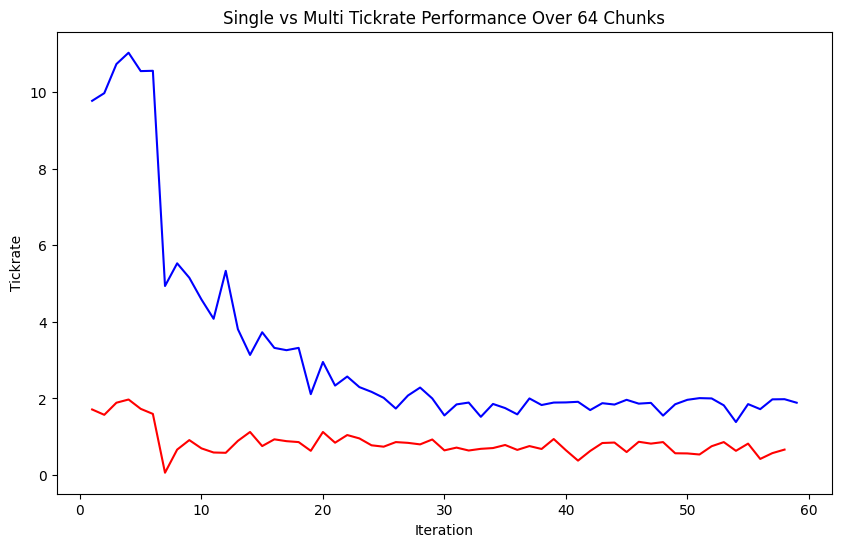
\includegraphics[width=0.65\linewidth]{resources/64chunks.png}
    \caption{Tick-rate comparison between single-thread vs multi-thread ECS a 1024 chunks}
    \label{fig:graph2}
\end{figure}

\begin{figure}[htbp]
    \centering
    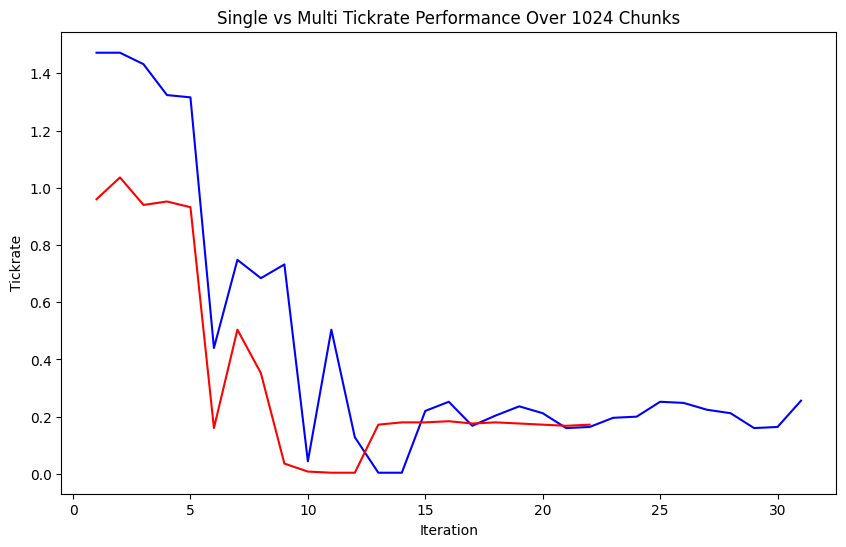
\includegraphics[width=0.65\linewidth]{resources/1024chunks.png}
    \caption{Tick-rate comparison between single-thread vs multi-thread ECS at 1024 chunks}
    \label{fig:graph2}
\end{figure}

